

This chapter describes how to compute the distance between the convex
hulls of two given point sets in $d$-dimensional Euclidean space
(\ccc{CGAL::Polytope_distance_d<Traits>}). Moreover, it is possible to
compute the width of a point set in three dimensions
(\ccc{CGAL::Width_3<Traits>}).

\begin{ccHtmlOnly}
<center>
<img border="0" src="polydist.gif" align="center">
</center>
\end{ccHtmlOnly} 

\begin{ccTexOnly}
\begin{center}
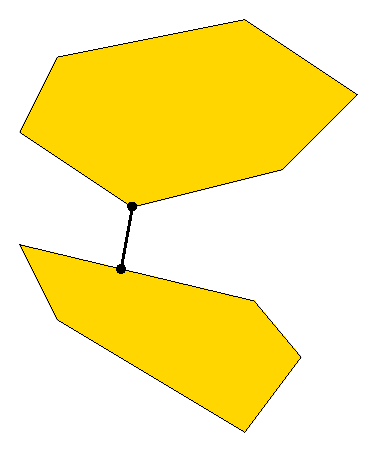
\includegraphics[width=4cm]{Optimisation/polydist}
\end{center}
\end{ccTexOnly}

The obvious application is collision detection between convex bodies
in space. In the spirit of the bounding volume application above, it
also makes sense for nonconvex objects: a full intersection test
between complicated objects could in a first stage be approximated
with the test between the convex hulls of the objects. Only if the
hulls intersect, a full intersection test is necessary.

To dampen fears concerning the performance of the distance
computation, we want to mention that the convex hulls of the input
point sets are not explicitly computed. This avoids a runtime which
grows exponentially in $d$. In fact, the runtime is almost always
linear in the size of the two point sets.

